% ─────────────────────────────────────────────────────────────────────────────
% SUPPLEMENTARY MATERIAL
% 3 figures (sup1–sup3) + 3 tables
% Counter \suppfigure increments for both figures and tables (S1–S6).
% ─────────────────────────────────────────────────────────────────────────────

% ─── S1: Experimental paradigm ───────────────────────────────────────────────
\begin{figure}[!h]
\centering
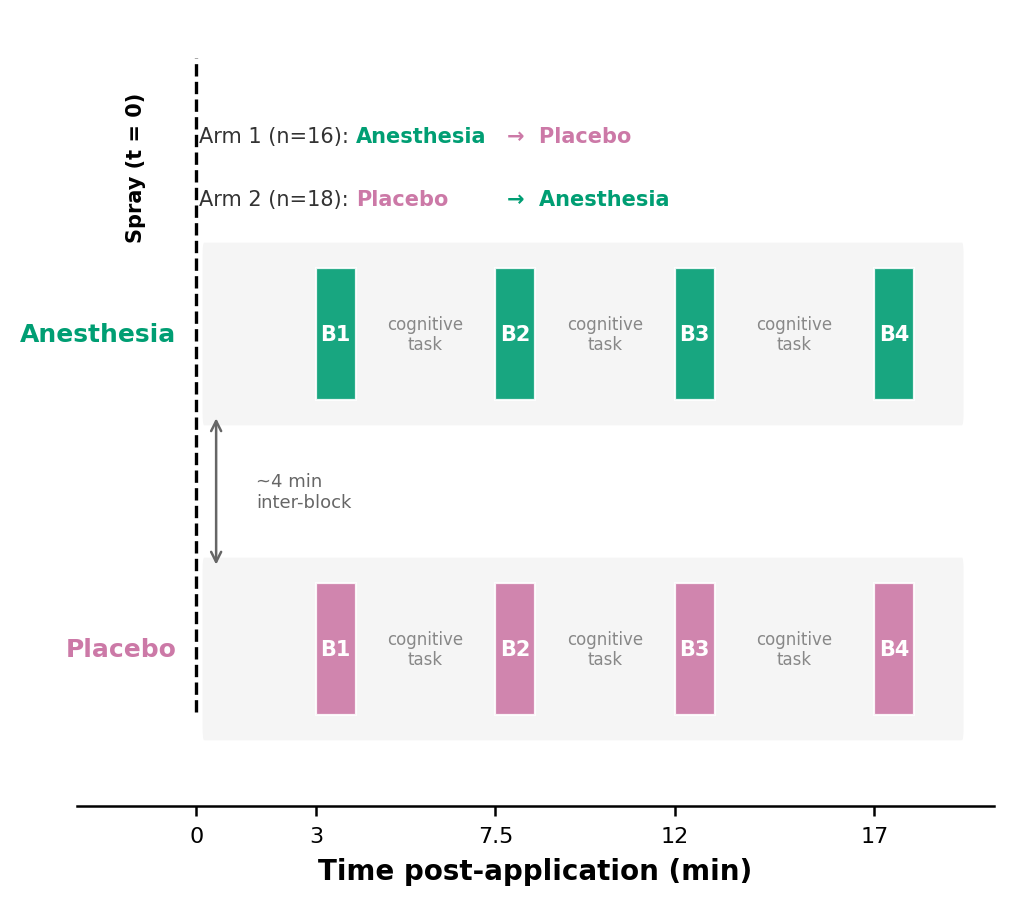
\includegraphics[width=\linewidth]{figures/sup1.png}
\refstepcounter{suppfigure}\label{fig:supp_paradigm}
\caption{\textbf{Supplementary Fig.~\thesuppfigure~$|$~Within-session
crossover design.}
Each experimental session comprised two chewing blocks separated by
$\approx$\,4~min.
Arm~1 ($n$\,=\,16): anesthesia block first, then placebo;
Arm~2 ($n$\,=\,18): placebo first, then anesthesia.
Each block began with a single spray application of topical lidocaine~10\%
or matched placebo (saline) at $t$\,=\,0; four 60-second chewing bouts
(B1--B4) commenced at approximately 3, 7.5, 12, and 17~min post-application.
Cognitive tasks (auditory oddball and 2-back) were performed between
consecutive bouts; these are indicated by the grey labels between blocks.
The short intra-session inter-block interval ($\approx$\,4~min) is sufficient
for pharmacological reversal: the placebo bout-1 is statistically equivalent
between arms (Supplementary Table~S3; carryover $p$\,=\,0.379; no period
effect $p$\,=\,0.134).
Green blocks: anesthesia condition; lilac blocks: placebo condition.}
\end{figure}

% ─── S2: Signal quality and participant inclusion ─────────────────────────────
\begin{figure}[!h]
\centering
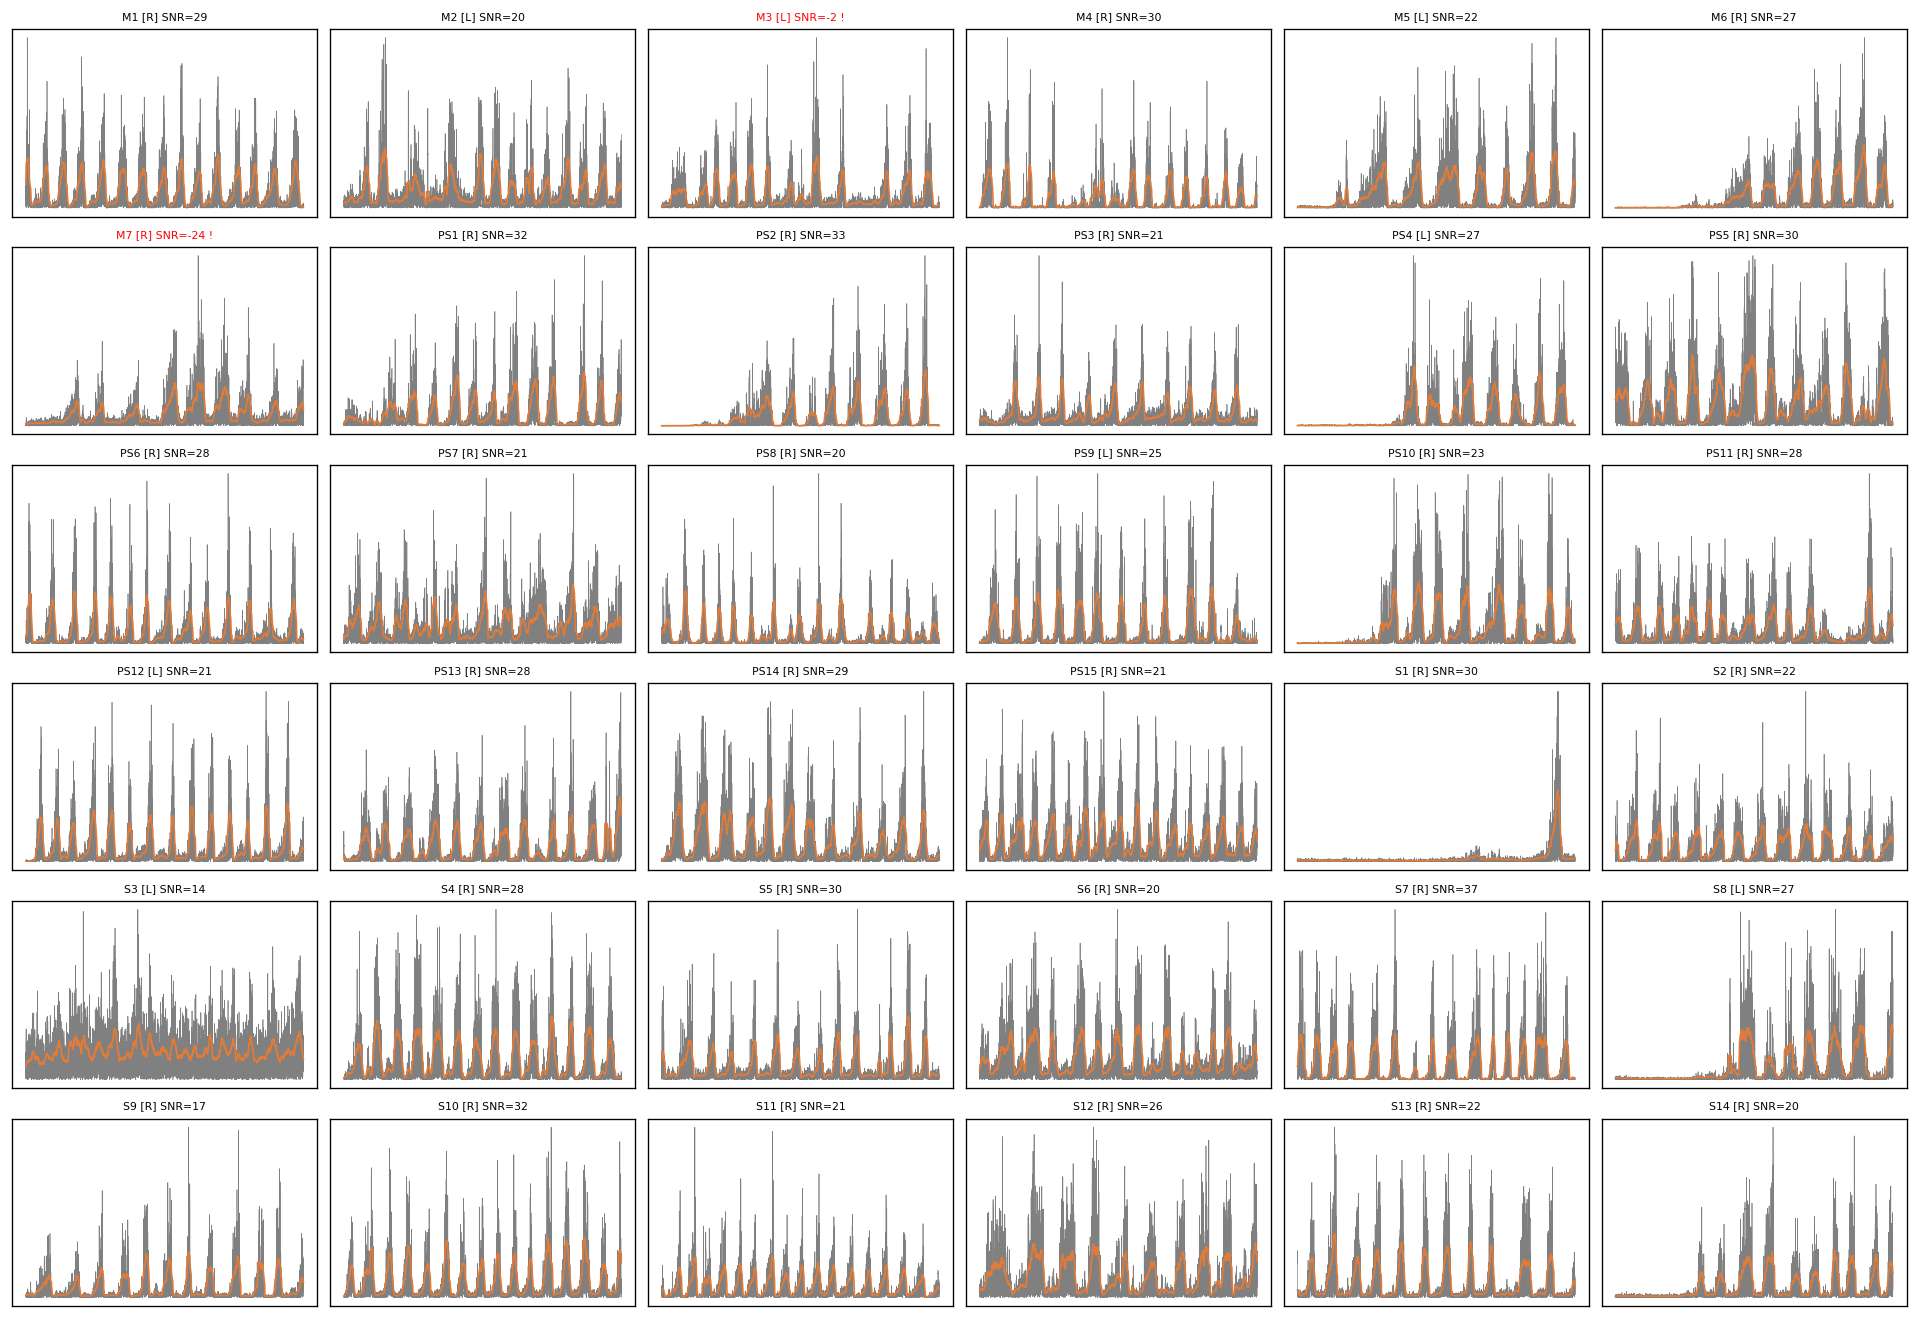
\includegraphics[width=\linewidth]{figures/sup2.png}
\refstepcounter{suppfigure}\label{fig:supp_qc}
\caption{\textbf{Supplementary Fig.~\thesuppfigure~$|$~Signal quality and
participant inclusion.}
Bipolar masseter EMG quality-control (QC) grid for all 36 recorded
participants.
Each panel shows the rectified bipolar waveform during the first 8~s of
chewing bout~1 (anesthesia and placebo overlaid) with detected cycle peaks
marked.
Two participants (M3, M7) are excluded from all analyses due to a dead
electrode in one condition, confirmed by near-zero amplitude and flat power
spectrum in the affected condition (SNR\,$<$\,3~dB).
Included: $N$\,=\,34; excluded: $N$\,=\,2.
Side selection (left or right masseter) was based on signal quality and
confirmed by automated SNR criterion.}
\end{figure}

% ─── S3: Effect-size overview and magnitude of change ────────────────────────
\begin{figure}[!h]
\centering
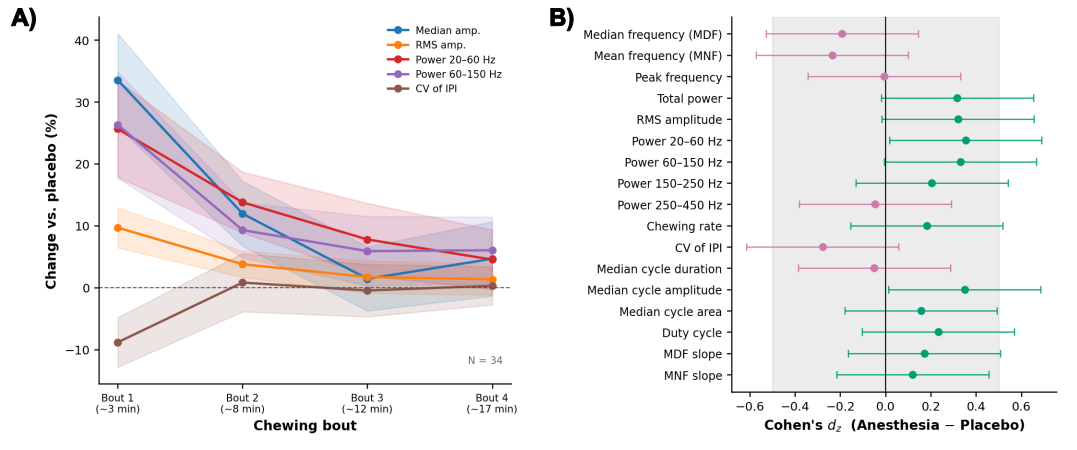
\includegraphics[width=\linewidth]{figures/sup3.png}
\refstepcounter{suppfigure}\label{fig:supp_effectsize}
\caption{\textbf{Supplementary Fig.~\thesuppfigure~$|$~Effect-size overview
and normalised magnitude of anesthesia-induced changes.}
\textbf{(A)} Percentage change relative to placebo
[(ANE\,$-$\,PLA)\,/\,$|$PLA$|$\,$\times$\,100] across chewing bouts~1--4 for
the five metrics with FDR-corrected significance at bout~1 (median amplitude,
RMS amplitude, power 20--60~Hz, power 60--150~Hz, CV\textsubscript{IPI}).
All metrics show a transient effect peaking at bout~1 ($\approx$\,3~min
post-application) that converges toward zero by bouts~3--4, consistent with
lidocaine pharmacokinetic washout.
Error bands: $\pm$\,SEM.
\textbf{(B)} Forest plot of Cohen's $d_z$ (ANE\,$-$\,PLA) for all 11 EMG
metrics, session-averaged across bouts~1--4.
Dots: point estimate; horizontal bars: 95\% CI ($\pm$\,1.96\,/\,$\sqrt{N}$).
The grey band marks the equivalence zone ($|d_z|$\,<\,0.5).
Session-averaged amplitude metrics are non-significant after FDR correction
(bout-1 effect diluted by within-session washout); timing and frequency
metrics lie within the equivalence band at all bouts, confirming the
gain--timing dissociation described in the main text.
$N$\,=\,34.}
\end{figure}

% ─────────────────────────────────────────────────────────────────────────────
% SUPPLEMENTARY TABLES
% ─────────────────────────────────────────────────────────────────────────────

% ─── S4: Session-averaged equivalence (TOST) ─────────────────────────────────
\refstepcounter{suppfigure}\label{fig:supp_tost}
\begin{table}[!h]
\centering
\caption{\textbf{Supplementary Table~\thesuppfigure~$|$~Session-averaged
anesthesia vs.\ placebo comparison (all four bouts pooled, $N$\,=\,34).}
Paired Cohen's $d_z$, Wilcoxon $p$, FDR-corrected $p$~\cite{Benjamini1995},
and two one-sided test (TOST) result at equivalence bound $|d|\,=\,0.5$~\cite{Lakens2017}.
TOST\,=\,Equiv.: both one-sided tests $p$\,<\,0.05.
Timing metrics satisfy or approach equivalence; amplitude metrics are
non-significant after FDR correction but do not satisfy equivalence,
consistent with the diluted transient effect described in the main text.}
\label{tab:tost_full}
\begin{tabular}{llrrrr}
\toprule
Category & Metric & $d_z$ & Wilcoxon $p$ & FDR $p$ & TOST ($|d|\leq0.5$) \\
\midrule
\multirow{5}{*}{Timing / frequency}
 & Median frequency (MDF)     & $-$0.191 & 0.186 & 0.376 & Equiv. \\
 & Mean frequency (MNF)       & $-$0.235 & 0.138 & 0.336 & Marginal ($p$\,=\,0.066) \\
 & Chewing rate (Hz)          & $+$0.182 & 0.278 & 0.415 & Equiv. \\
 & Cycle duration (s)         & $-$0.049 & 0.758 & 0.806 & Equiv. \\
 & Duty cycle                 & $+$0.233 & 0.221 & 0.376 & Marginal ($p$\,=\,0.065) \\
\midrule
\multirow{6}{*}{Amplitude / power}
 & Median cycle amplitude     & $+$0.349 & 0.011 & 0.181 & Not equiv. \\
 & RMS amplitude              & $+$0.320 & 0.109 & 0.336 & Not equiv. \\
 & Total power                & $+$0.317 & 0.109 & 0.336 & Not equiv. \\
 & Power 20--60~Hz            & $+$0.354 & 0.121 & 0.336 & Not equiv. \\
 & Power 60--150~Hz           & $+$0.331 & 0.109 & 0.336 & Not equiv. \\
 & CV inter-peak interval     & $-$0.278 & 0.046 & 0.336 & Not equiv. \\
\bottomrule
\end{tabular}
\end{table}

% ─── S5: Bout-resolved statistics ────────────────────────────────────────────
\refstepcounter{suppfigure}\label{fig:supp_boutstats}
\begin{table}[!h]
\centering
\caption{\textbf{Supplementary Table~\thesuppfigure~$|$~Bout-resolved
anesthesia vs.\ placebo effect sizes ($d_z$, paired Cohen's~$d$~\cite{Cohen1988})
for key metrics, $N$\,=\,34.}
FDR $p$ shown only for bout~1 (Benjamini--Hochberg~\cite{Benjamini1995} across
11 metrics); asterisks denote FDR-corrected significance (**\,$p$\,<\,0.01;
*\,$p$\,<\,0.05).
Interaction $p$: Greenhouse--Geisser-corrected condition\,$\times$\,bout
repeated-measures ANOVA~\cite{Pingouin}.
Positive $d_z$ = ANE\,$>$\,PLA; negative $d_z$ for CV\textsubscript{IPI}
indicates greater regularity under anesthesia.}
\label{tab:bout_stats}
\begin{tabular}{lrrrrrr}
\toprule
Metric & \multicolumn{4}{c}{$d_z$ by bout} & FDR $p$ (b1) & Inter. $p$ \\
\cmidrule(lr){2-5}
       & Bout 1 & Bout 2 & Bout 3 & Bout 4 & & \\
\midrule
\textit{Amplitude}\\
\quad Median cycle amplitude & $+$0.695** & $+$0.248 & $-$0.120 & $-$0.058 & 0.0035 & 0.0010 \\
\quad RMS amplitude          & $+$0.487*  & $+$0.257 & $+$0.034 & $+$0.024 & 0.0132 & 0.130  \\
\quad Total power            & $+$0.456*  & $+$0.261 & $+$0.032 & $+$0.095 & 0.0132 & 0.260  \\
\quad Power 60--150~Hz       & $+$0.463*  & $+$0.281 & $+$0.025 & $+$0.100 & 0.0189 & 0.238  \\
\quad Power 20--60~Hz        & $+$0.467*  & $+$0.231 & $+$0.151 & $+$0.027 & 0.0274 & 0.445  \\
\midrule
\textit{Regularity}\\
\quad CV\textsubscript{IPI}  & $-$0.434*  & $-$0.051 & $-$0.070 & $-$0.026 & 0.0415 & 0.057  \\
\midrule
\textit{Timing (all non-significant; TOST-equivalent at all bouts)}\\
\quad Median frequency (MDF) & $-$0.147 & $-$0.275 & $-$0.139 & $+$0.085 & 0.621 & 0.485 \\
\quad Chewing rate           & $+$0.054 & $+$0.331 & $-$0.069 & $+$0.113 & 0.919 & 0.230 \\
\quad Duty cycle             & $+$0.045 & $+$0.203 & $+$0.213 & $+$0.185 & 0.909 & 0.848 \\
\bottomrule
\end{tabular}
\end{table}

% ─── S6: Robustness ──────────────────────────────────────────────────────────
\refstepcounter{suppfigure}\label{fig:supp_robust}
\begin{table}[!h]
\centering
\caption{\textbf{Supplementary Table~\thesuppfigure~$|$~Robustness of the
bout-1 anesthesia effect across inclusion cohorts.}
Bout-1 paired Cohen's $d_z$, Wilcoxon $p$, percentage of participants with
ANE\,$>$\,PLA, and condition\,$\times$\,bout RM-ANOVA interaction $p$
(Greenhouse--Geisser corrected) for median cycle amplitude under four
alternative inclusion thresholds.
The attenuation at $N$\,=\,36 is attributable to M3 and M7 (dead electrode in
one condition), whose inclusion approximately halves the effect size while the
paired test remains significant ($p$\,=\,0.002), confirming the
quality-based exclusion criterion.}
\label{tab:robustness}
\begin{tabular}{lrrrrr}
\toprule
Cohort & $N$ & $d_z$ & Wilcoxon $p$ & \%~ANE$>$PLA & cond$\times$bout $p$ \\
\midrule
QC automatic                     & 34 & 0.69 & 0.0003 & 76\% & 0.0004 \\
Lista~30                         & 30 & 0.68 & 0.001  & 77\% & 0.001  \\
Lista~32                         & 32 & 0.65 & 0.001  & 75\% & 0.001  \\
All (incl.\ M3/M7, $N$\,=\,36)  & 36 & 0.26 & 0.002  & 72\% & 0.061  \\
\bottomrule
\end{tabular}
\end{table}
